% =====================================================================
%  Phan ly thuyet viet lai -- TETC-2026-05-0252
%  Tra loi R3-3 (proposition la su that hien nhien), R4 (Theorem 1 sai,
%  Pareto khong loc gi, Proposition 3 khong duoc dan xuat).
%
%  Thay the trong ban da nop:
%    - Proposition 1, 3, 4  -> ha xuong Fact/Remark co trich dan, bo proof
%    - Proposition 2        -> doi thanh Lemma 1, proof chuyen xuong phu luc
%    - Definition 4 (Pareto), Algorithm 1, Eq. (6) J(n), Theorem 1 -> BO HAN
%    - Thay bang luat ba giai doan tu vung (lexicographic), khong co trong so
%
%  Anh xa cite key -> so tai lieu cua ban da nop (KHONG them ref moi):
%    cortes1995=[16] Cortes&Vapnik   scholkopf2002=[17] Scholkopf&Smola
%    havlicek2019=[11]               schuld2019=[12] Schuld&Killoran
%    thanasilp2024=[22]              cortes2012=[23] Cortes,Mohri,Rostamizadeh
%    cristianini2002=[28]
% =====================================================================

% ---------------------------------------------------------------------
% III-B  Preliminaries -- khong con proposition/proof cho su that hien nhien
% ---------------------------------------------------------------------
\subsection{Preliminaries}

We use three standard facts, stated here for reference rather than proved,
since each is established in the literature.

\begin{enumerate}
  \item[\textbf{(F1)}] \emph{Positive semi-definiteness.} For any finite sample,
    the Gram matrix $[K^{\mathrm{Q}}(\bm{x}_i,\bm{x}_j)]_{i,j=1}^{N}$ induced by
    a feature map is symmetric and positive semi-definite, being a Hadamard
    product of two Hermitian PSD factors, by the Schur product
    theorem \cite{scholkopf2002}. This is what licenses the use of
    $K^{\mathrm{Q}}$ inside the dual soft-margin SVM
    \cite{cortes1995,scholkopf2002}, with the quantum kernel slotting in exactly
    as in \cite{havlicek2019,schuld2019}.
  \item[\textbf{(F2)}] \emph{Kernel--target alignment and generalisation.}
    Higher alignment together with comparable empirical risk implies a tighter
    generalisation bound \cite{cristianini2002,cortes2012}; we use the bound
    exactly as stated in \cite{cortes2012} and derive nothing new from it. Its
    role here is diagnostic: two kernels with the same empirical risk may differ
    in the bound because the hypothesis classes their geometries induce differ.
  \item[\textbf{(F3)}] \emph{Concentration at large width.} Fidelity kernels
    built from expressive feature maps concentrate toward a constant as the
    number of qubits grows \cite{thanasilp2024}, which is an independent reason
    --- beyond gate count --- to prefer a small embedding dimension.
\end{enumerate}

\begin{remark}
In the submitted version these three facts appeared as Propositions~1, 3 and~4
with accompanying proofs. We agree with the reviewer that presenting established
results in that form was inappropriate, and that the proof of the former
Proposition~3 restated \cite{cortes2012} rather than deriving anything. They are
now cited as background.
\end{remark}

% ---------------------------------------------------------------------
% II-B  Lemma 1 -- day la dan xuat rieng cua bai, nen giu, chi doi ten
% ---------------------------------------------------------------------
\begin{lemma}[Local expansion of the \ZZ{} kernel at $r=1$]
\label{lem:expansion}
Let $r=1$ and let $\bm{x},\bm{x}^{\prime}\in[0,\pi]^n$ with $\bm{x}^{\prime}$
sufficiently close to $\bm{x}$. Then the kernel of Eq.~\eqref{eq:kernel} admits
the second-order expansion
\begin{equation}
\label{eq:expansion}
  K^{\mathrm{Q}}(\bm{x},\bm{x}^{\prime}) \;=\; 1
  - \sum_{i=1}^{n}\Delta_i^2
  - \tfrac{1}{4}\!\!\sum_{1\le i<j\le n}\!\!\Delta\varphi_{ij}^2
  + O(\|\bm{x}-\bm{x}^{\prime}\|^4),
\end{equation}
where $\Delta_i := x_i - x_i^{\prime}$ and
$\Delta\varphi_{ij} := \varphi_{ij}(\bm{x}) - \varphi_{ij}(\bm{x}^{\prime})$.
\end{lemma}

\begin{remark}[The expansion does not extend to $r\ge2$]
\label{rem:reps}
The restriction to one repetition is not cosmetic. For $r\ge2$ the interleaved
Hadamard layers make $U_{\Phi}(\bm{x}^{\prime})^{\dagger}U_{\Phi}(\bm{x})$
non-diagonal and no pair of coefficients renders the two-invariant form correct:
a least-squares fit at $r=2$ attains only $R^2=0.60$--$0.94$, with coefficients
that change sign between expansion points. The quantity $1-K^{\mathrm{Q}}$
stays a quadratic form in $\bm{x}-\bm{x}^{\prime}$ at every $r$ (fitting to
$R^2>0.999$) but is no longer expressible in these two invariants. Since our
operating point is $r=2$, we use Lemma~\ref{lem:expansion} for the structural
reading below and not as a numerical statement. See
\texttt{runners/verify\_lemma1.py}.
\end{remark}

Lemma~\ref{lem:expansion} is retained because, unlike (F1)--(F3), it is specific
to the comparison this paper makes: the linear part $\sum_i \Delta_i^2$ is the
quantity a Gaussian RBF kernel controls through its bandwidth, and the pairwise
part expands into the monomials a degree-2 polynomial kernel can represent. What
the classical kernels lack is the higher-order oscillation carried by the
exponentials, bounded above by~1 because $K^{\mathrm{Q}}$ is a squared fidelity
whereas the polynomial inner product grows unboundedly with $\|\bm{x}\|$. This is
why SVM-\textsc{Poly2} is the sharpest classical comparator, and
Sec.~\ref{sec:res-c2} confirms that it is. The proof is given in
Appendix~\ref{app:lemma}.

% ---------------------------------------------------------------------
% III-C  Luat chon so chieu -- THAY HAN cho Pareto + J(n) + Theorem 1
% ---------------------------------------------------------------------
\subsection{C1: A Three-Stage Rule for the Embedding Dimension}

% Sinh boi runners/make_paper1_figures.py; caption doi chieu bang
% runners/audit_figures.py. File rieng cho tung hinh de \input DUNG CHO
% trong than bai -- float cua LaTeX chi troi VE SAU, khai bao het o cuoi
% tai lieu thi ca 9 hinh don xuong cuoi va tran vao danh muc tai lieu.

\begin{figure*}[t]
  \centering
  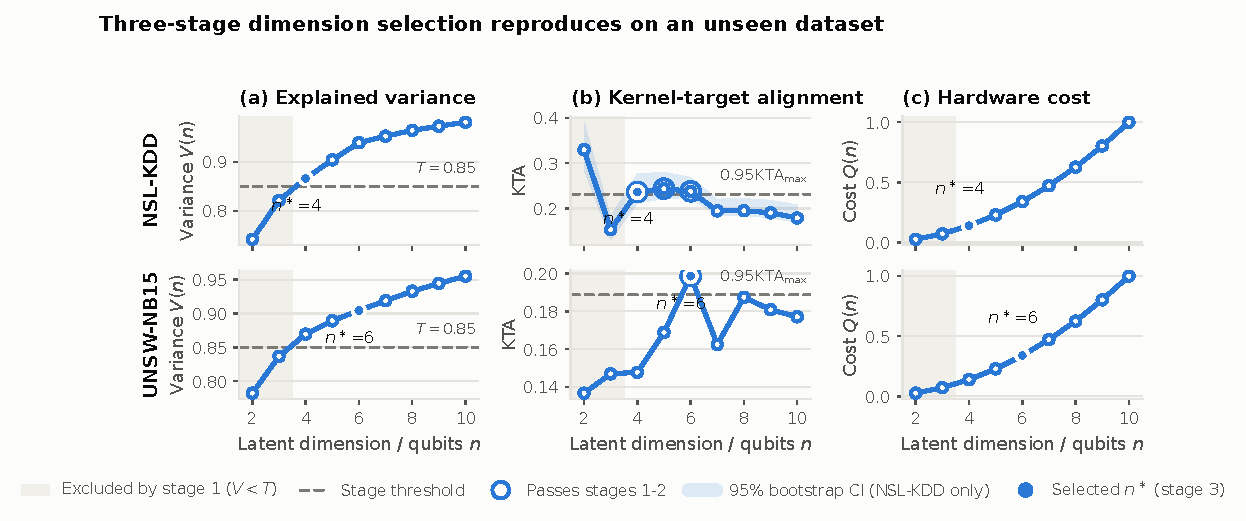
\includegraphics[width=\textwidth]{figs_revision/fig5_c1_dimension_selection.pdf}
  \caption{%
    \textbf{The three-stage dimension-selection rule, applied unchanged to two
    datasets.} Rows: NSL-KDD (top), UNSW-NB15 (bottom). Columns: (a) cumulative
    explained variance $V(n)$, (b) kernel--target alignment, (c) CNOT-weighted
    cost $Q(n)$. Stage~1 discards $V(n)<0.85$ (shaded), stage~2 keeps
    $\mathrm{KTA}\ge0.95\,\mathrm{KTA}_{\max}$ (open circles), stage~3 takes the
    cheapest survivor (filled). The same rule returns $n^{\ast}=4$ and
    $n^{\ast}=6$.}
  \label{fig:c1-selection}
\end{figure*}


The submitted version selected $n$ by Pareto filtering followed by a weighted
scalarisation $J(n) = \alpha V(n) + \beta\widetilde{F}(n) - \gamma Q(n)$. That
construction has been removed; Sec.~\ref{sec:erratum} states why. It is replaced
by a rule that is \emph{lexicographic} rather than compensatory, so no weights
are involved and no trade-off among the three objectives has to be asserted.

\begin{definition}[Three-stage selection]
\label{def:three-stage}
Let $\mathcal{N}$ be the candidate set, $V(n)$ the cumulative explained variance,
$\mathrm{KTA}(n)$ the kernel--target alignment of the induced Gram matrix, and
$Q(n)$ the CNOT-weighted cost of Eq.~\eqref{eq:cost}. Fix $T=0.85$ and $\epsilon=0.05$
\emph{before} inspecting any downstream metric. Then
\begin{align}
  \mathcal{N}_1 &:= \{\, n \in \mathcal{N} : V(n) \ge T \,\}, \\
  \mathcal{N}_2 &:= \Bigl\{\, n \in \mathcal{N}_1 : \mathrm{KTA}(n) \ge
                   (1-\epsilon)\!\!\max_{m\in\mathcal{N}_1}\!\mathrm{KTA}(m)
                   \,\Bigr\}, \\
  n^{\ast}      &:= \arg\min_{n \in \mathcal{N}_2} Q(n).
\end{align}
\end{definition}

The three stages ask three different questions and are therefore not
interchangeable. Stage~1 asks whether the representation still carries the
signal; stage~2 asks whether the \emph{kernel} on that representation is aligned
with the labels; stage~3 breaks the remaining tie by hardware cost. Stage~1 is
what removes $n=2$ on NSL-KDD despite its being the most aligned candidate
overall: a kernel can be well aligned on a representation that has already
discarded a quarter of the variance.

On NSL-KDD the rule gives $\mathcal{N}_1=\{4,\dots,10\}$, a maximum alignment of
$0.2439$ at $n=5$, hence a stage-2 threshold of $0.2317$, $\mathcal{N}_2=\{4,5,6\}$
and $n^{\ast}=4$. Applied unchanged to UNSW-NB15 it gives $\mathcal{N}_2=\{6\}$
and $n^{\ast}=6$, recovered on $10/10$ independent subsets and under every
threshold perturbation we tested (Fig.~\ref{fig:c1-selection}). We therefore
present C1 as a transferable \emph{procedure} whose output is a property of the
dataset, and not as the constant $n=4$.

% ---------------------------------------------------------------------
% III-D  Thay z-test cua Proposition 4 bang giao thuc ghep cap
% ---------------------------------------------------------------------
\subsection{Identifying the Entanglement Contribution}

The submitted version certified the entanglement effect with a two-sample
$z$-test over $m=5$ subsets (former Proposition~4). Two things are wrong with
that. The test treats the two arms as independent when they in fact share the
training subset, discarding the pairing that makes the comparison informative;
and five subsets is too few for the normal approximation it invokes.

The revision compares the arms \emph{pairwise within a run}. For each of ten runs
we compute
$\Delta = \mathrm{KTA}_{\mathrm{ZZ}} - \mathrm{KTA}_{\mathrm{Z}}$ on the same
subset and report the mean with a $t$-based 95\% interval, a Wilcoxon
signed-rank test, and the paired effect size $d_z$. Because each contribution
tests several baselines, $p$-values are Holm-corrected within baseline families
(\emph{entanglement}, \emph{classical kernel}, \emph{strong tabular}), and every
verdict reported in this paper is the corrected one. This is strictly more
conservative than the former $z$-test and assumes nothing beyond symmetry of the
paired differences.

% ---------------------------------------------------------------------
% Erratum -- phai noi thang, khong de reviewer tu tim ra
% ---------------------------------------------------------------------
\subsection{Corrections to the Submitted Version}
\label{sec:erratum}

Four defects in the submitted theory section are corrected here; two were
identified by reviewers and two we found ourselves, and we report them on the
same footing. The accompanying letter gives the full derivations.

\textbf{(i) Theorem~1 was false.} Its proof asserted
$\widetilde{F}(4) > \widetilde{F}(3)$, whereas Table~III of the same submission
reports $0.471 < 0.628$. With the correct values the objective is maximised at
$n=2$ $(J=0.551)$, not at $n=4$. We thank the reviewer for identifying this.

\textbf{(ii) The Pareto stage filtered nothing.} $V(n)$ increases monotonically
while $\widetilde{F}(n)$ decreases and $Q(n)$ increases, so every candidate is
Pareto-optimal. Theorem~1 and $J$ are removed rather than repaired, because this
second defect shows the construction was not doing the work attributed to it.

\textbf{(iii) The former Proposition~2 had incorrect coefficients.} It asserted
the expansion with $r^{2}$ on both sums. The correct weights are $1$ and
$\tfrac{1}{4}$ (Lemma~\ref{lem:expansion}), and the $r^{2}$ prefactor does not hold
at all for $r\ge2$ (Remark~\ref{rem:reps}). The difference is not marginal: with
the submitted coefficients the residual decays as $\|\cdot\|^{2}$ rather than
$\|\cdot\|^{4}$, so the claimed second-order accuracy is not attained. No reviewer
raised this; we found it while transcribing the proof. The consequence drawn
from it --- that SVM-\textsc{Poly2} is the sharpest classical comparator --- is
unaffected, depending on which monomials appear and not on their coefficients.

\textbf{(iv) Table~III mislabelled its third column.} The caption defined
$\widetilde{F}(n)=1/\mathrm{DBI}(n)$, but the tabulated values are the ANOVA
$F$~statistic. No conclusion depends on it, the quantity having been dropped
along with $J$, but we record it for completeness.
